\section{Fremgangsmetode}

\section{Måling af cellespændinger}
Systemet er til hver en tid nødt til at kende den samlede cellespænding, for at vide hvornår opladning er nødvendig. Da systemet samtidig skal være i stand til at måle de individuelle cellespændinger under opladning, er det derfor smart, at sætte en spændingsmåler hen over hver celle. På den måde kan de enkelte celler måles og batteripakkens udgangsspænding kan fås ved addition af alle celler.
\\

Måling af cellespænding kan opnås ved brug af en differensforstærker, for at få spændingsforskellen mellem hver celle. Outputtet af forstærkeren kan efterfølgende sendes ind i microens ADC. Da en celle kan variere mellem $3.2\volt$ og $4.2\volt$, samtidig med at microen er forsynet med $3.3\volt$, skal differensforstærkeren dimensioneres derefter. I praksis kan dette løses ved at have et gain på mindre end 1, for at få outputtet til at svinge på til microens forsyningsspænding ved maksimal cellespænding.
\\



\section{Strømmåling}
For at overvåge udgangsstrømmen skal en strømmåler realiseres. Dette kan gøres ved hjælp af en shunt modstand, $R_{s}$, som yder en meget lille og veldefineret ohmsk belastning og kan holde til hele udgangsstrømmen. Når belastningen trækker en strøm, vil et lille spændingsfald forekomme over shunt modstanden, som en differensforstærker vil detektere. 


Shunt modstanden kan både placeres på høj- og lavsiden, som illustreret på figur XXX
\klp{Illustration af shunt placering}



På figur \ref{fig:current_sense} ses schematics over strømmåleren.
\begin{figure}[h]
	\centering
	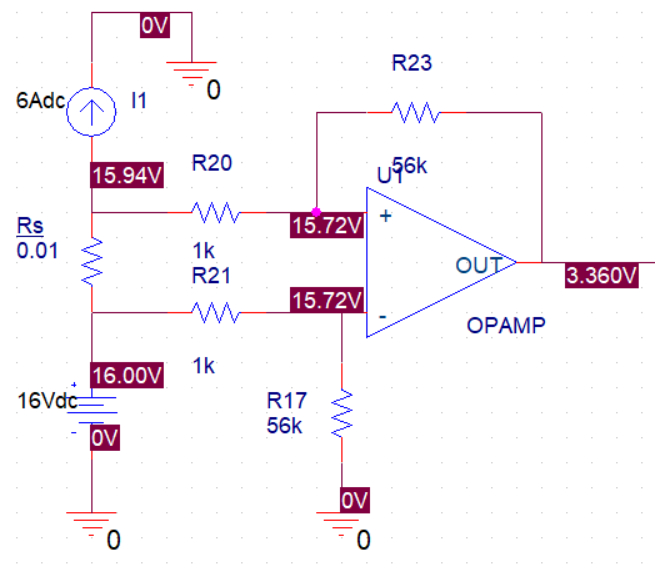
\includegraphics[width=15cm]{billeder/current_sense.png}
	\caption{Differensforstærker som strømmåler}
	\label{fig:current_sense}
\end{figure}

En vigtig parameter under dimensionering af en strømmåler er valg af shunt modstandens værdi. Ud fra den maksimale afladestrøm $I_{out} = 6\ampere$ vælges shunt modstanden $R_{s} = 10\milli\ohm$. Det maksimale spændingsfald, $V_{s}$ over shunt modstanden bliver derfor
\begin {equation} 
V_{s} = R_{s} * I_{out} = 10\milli\ohm * 6\ampere = 60\milli\volt
\end {equation}

Afladestrømmen kan variere mellem $0\ampere$ og $6\ampere$, så spændingsfaldet vil ligge mellem $0\milli\volt$ og $60\milli\volt$. Da microcontrolleren kører med en logik på $3.3\volt$ og har en ADC med en opløsning på 12 Bit, skal signalet dimensioneres efter dette. Ved hjælp af en differensforstærker kan et brugbart indgangssignal til ADC'en realiseres. Forstærkeren er opbygget med en operationsforstærker koblet med positiv feedback.
\\

Den nødvendige forstærkning $A_{v}$ af signalet findes,
\begin {equation} 
A_{v} = \frac{V_{o}}{V_{s}} = \frac{3.3\volt}{60\milli\volt} = 55
\end {equation}

For at opnå denne forstærkning anvendes en

\subsubsection{Realisering af shunt modstand}
For at gøre målingen så 
\begin {equation} 
V_{out} = \frac{R_{1}+R_{2}}{R_{3}+R_{4}} = \frac{3.3\volt}{60\milli\volt} = 55
\end {equation}
\section{Passiv balancering}

\section{Driverkreds til styring af MOSFETs}
Lade og aflade fet

If N-Channel MOSFETs are used on the pack + side, the IC needs to have a charge pump that can provide a gate voltage higher than the battery voltage.  Most simple protection ICs will not have a charge pump so then there are 2 options:

Use N-Channel MOSFETs on the pack – side to disconnect the battery.  The disadvantage here is that you need to understand and mitigate the impact to the system when the battery ground is disconnected.
Use P-Channel MOSFETs on the pack + side to disconnect the battery.  P-Channel MOSFETs are not as common as N-Channel and selection may not be great. They are usually more expensive than N-Channel.

De er begge altid ON

\section{Sikkerhed ved overstrøm}
Lidt forord

For at undgå, at strømmåleren oscillerer kan en Set-reset flipflop ...
\subsection{Overstrøm ved afladning}


Da en overstrøm også kan forekomme ved kortslutning af udgangsterminalerne, vil den derfor også trigge på det.

\subsection{Overstrøm ved opladning}

\section{Spændingsnet}
Forsyningsspændingen til hele BMS'en kommer fra batteripakkens terminalspænding, som kan variere mellem $12.4\volt - 16.8\volt$. For at generere to nødvendige netspændinger på $12\volt$ og $3.3\volt$, skal to spændingsregulatorer realiseres.
\\

For 

